\documentclass[tikz,border=2pt]{standalone}
\usepackage{amsmath,amssymb}
\usepackage{pgfplots}
\pgfplotsset{compat=1.18}

\begin{document}
% Negative binomial pmf (r = 3, p = 0.4): the number of trials needed for the 3rd success; the
% support starts at k = r and the mass sits around r/p = 7.5.
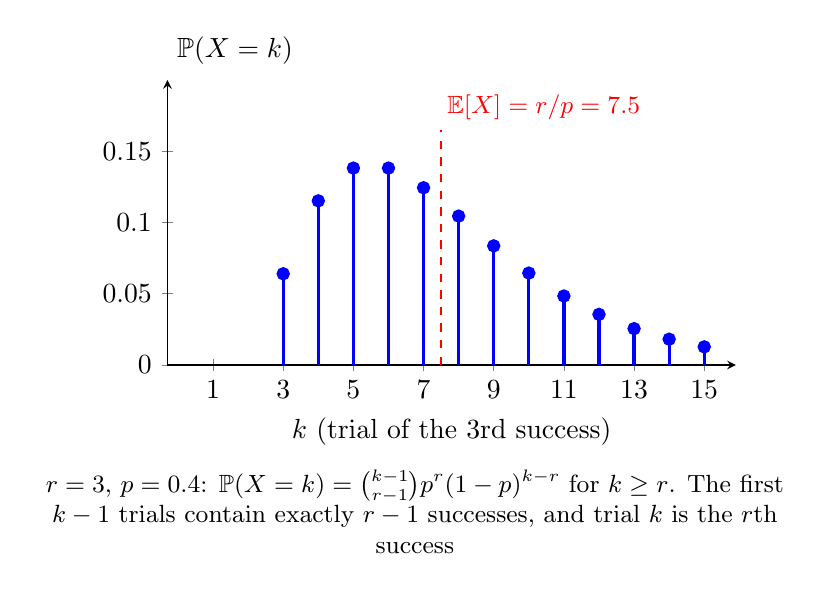
\begin{tikzpicture}
	\begin{axis}[
		axis lines=left, xmin=-0.3, xmax=15.9, ymin=0, ymax=0.2,
		xtick={1,3,5,7,9,11,13,15}, ytick={0,0.05,0.1,0.15},
		yticklabel style={/pgf/number format/fixed, /pgf/number format/precision=2}, scaled y ticks=false,
		xlabel={$k$ (trial of the $3$rd success)}, ylabel={$\mathbb{P}(X=k)$}, ylabel style={rotate=-90, anchor=south west, at={(axis description cs:0,1.02)}},
		width=8.8cm, height=5.2cm, clip=false
		]
		\addplot[ycomb, blue, very thick, mark=*, mark size=1.8pt] coordinates {(3,0.0640) (4,0.1152) (5,0.1382) (6,0.1382) (7,0.1244) (8,0.1045) (9,0.0836) (10,0.0645) (11,0.0484) (12,0.0355) (13,0.0255) (14,0.0181) (15,0.0127)};
		\draw[red, dashed, thick] (axis cs:7.5,0) -- (axis cs:7.5,0.165);
		\node[red, anchor=south west, font=\small] at (axis cs:7.4,0.165) {$\mathbb{E}[X]=r/p=7.5$};
	\end{axis}
	\node[anchor=north, font=\small, align=flush center, text width=9.6cm] at ([yshift=-2pt]current axis.outer south) {$r=3$, $p=0.4$: $\mathbb{P}(X=k)=\binom{k-1}{r-1}p^r(1-p)^{k-r}$ for $k\ge r$. The first $k-1$ trials contain exactly $r-1$ successes, and trial $k$ is the $r$th success};
\end{tikzpicture}
\end{document}
